%-----------------------------------------------------------------------------
%
%          PHYSICS  M.S.     THESIS
%          JUSTIN A. VASEL
%
%          This began as the template offered by the University of Minnesota, 
%          but I've made a few changes here and there...  
%
%          -->  neutrinos.tex
%
%-----------------------------------------------------------------------------


\chapter{The Physics of Neutrinos}
	\label{neutrino_physics_chapter}

	\vspace{-0.2in}

	\begin{quoting}
		\noindent \large ``Neutrinos, they are very small." \normalsize

		--- John Updike
	\end{quoting}

	\chapterIntro{T}{he turn of the twentieth century} marked the beginning of a golden age in physics. The formulation of relativity and formalism of quantum mechanics brought with it a wealth of paradigm-shifting discoveries, offering humanity a deeper, more fundamental understanding of the Universe and paving the way for decades of ground-breaking research. One of the crowning achievements of this era has been the construction of the Standard Model of particle physics.

	The advent of the model was paramount to the advancement of modern physics. Through its theoretical framework, the particle physicist can calculate, among other things: decay modes, branching ratios and intrinsic properties of a myriad of particles. In some instances, the very existence of yet unobserved particles can be inferred from the Standard Model. The prediction of the Higgs boson---whose existence was proposed to preserve gauge invariance---is perhaps the most notable example, being initially theorized in 1964 and finally discovered in March 2013.

	It is essential in particle physics that one be able to predict the observed phenomena before it is observed. While atomic particles like the proton, neutron, and electron are easy to detect, many particles are not. This is especially true for particles that have a low mass or no charge, like the neutrino, or very brief lifetimes like the Higgs boson. It is nearly impossible to detect these particles directly. Instead, one must depend on indirect observations like the products of an interaction or the daughter particles of a decay sequence. To make new discoveries, the particle physicist must know what she is looking for and where she might find it; it is the nature of the beast. 

	\section{The Standard Model of Particles}

	The Standard Model of Particles is the result of large-scale scientific collaboration, spanning several continents and decades. Feynman said in his famous recorded lectures on physics that the goal of physics is first to observe and describe different types of phenomena and then amalgamate those phenomena into a larger, encompassing theory. The Standard Model is the result of such amalgamations, beginning with the unification of two of nature's fundamental forces: electromagnetism and the weak interaction. At high-enough energies---about \eGeV{100}, corresponding to a temperature of \SI{e15}{\kelvin}---the two forces become indistinguishable, forming the so-called electroweak interaction. Further unification of the fundamental forces has yet to be achieved, but the incorporation of the Higgs mechanism---which gives mass to elementary particles---and the understanding of the strong interaction has lead to the Standard Model that we know today.

	Sixty-one elementary particles are described by the Standard Model. They are elementary in the sense that they are not composed of more fundamental constituents. These particles consist of the quarks---of which there are thirty-six: (six quarks + six antiquarks) $\times$ three color charges per quark---twelve leptons, and thirteen force-carrying bosons.

	\subsection{Fermions}
	\label{sec:fermions}

	Fermions are a designation given to leptons and quarks. The \emph{leptons} are the electron, muon, tau particles and their associated neutrinos. The quarks are the up, down, charm, strange, top, and bottom. All of these particles have antiparticles, which are also fermions. Fermions are designated as such because they follow the laws of Fermi-Dirac statistics. Identical fermions obey the Pauli exclusion principle. 

	Three quarks together from \emph{baryons}, which are also fermionic particles. Examples include the proton and the neutron. A quark-antiquark pair is called a \emph{meson}, and somewhat counter-intuitively constitutes a bosonic particle, which will be discussed in greater depth in \SEC \ref{sec:bosons}. Any combination of quarks constitutes a \emph{hadron}.

	These elementary fermions---leptons and quarks---are categorized into three ordered generations, each generation being greater in mass than the one before it. There are two conserved quantities associated with fermions---The lepton quantum number and the baryon quantum number. Like momentum or energy, any process involving fermions must conserve these quantities. 

	\begin{table}[H]
		\centering
		\captionsetup{width=4in}
		\caption[The Elemenetary Fermions]{The elementary fermions are divided into generations. Mass increases from generation one to three. The first generation is the most stable.}
		\label{table:leptons}
		\begin{tabular}{cccc}
			\toprule
			 & First & Second & Third \\
			 & Generation & Generation & Generation \\
			\midrule
			\multirow{2}{*}{\emph{Leptons}} & \HepParticle{\Pelectron} & \HepParticle{\Pmu} & $\tau$ \\ 
			 & \HepParticle{\Pnue} & \HepParticle{\Pnum} & $\nu_{\tau}$ \\
			\midrule
			\multirow{2}{*}{\emph{Quarks}} & \HepParticle{\Pup}{}{} & \HepParticle{\Pcharm}{}{} & \HepParticle{\Ptop}{}{} \\
			 & \HepParticle{\Pdown}{}{} & \HepParticle{\Pstrange}{}{} & \HepParticle{\Pbottom}{}{} \\
			\bottomrule
		\end{tabular}
	\end{table}

	\subsection{Bosons}
	\label{sec:bosons}
	Bosons represent all matter that is not fermionic. They are so named because they obey Bose-Einstein statistics, the other pillar of the dichotomy that describes systems of particles. Like fermions, some bosons are elementary particles. These are the five force carriers: $\gamma$ (electromagnetic), $g$ (strong), $W^{\pm}$\&$Z$ (weak), and $H$ (Higgs). There are other bosons that are composite particles and they constitute the \emph{mesons}, mentioned briefly in \SEC \ref{sec:fermions}. These particles are composed of a quark-antiquark pair and are very unstable, quickly decaying into more stable fermions.

	The bosons have associated with them no conserved quantities and are not constrained by nearby particles in the states they can occupy. The bosons are also distinct is that the force carries mediate interactions between the other particles. 

	\noindent
	\begin{wrapfigure}{l}{0.3\textwidth}
		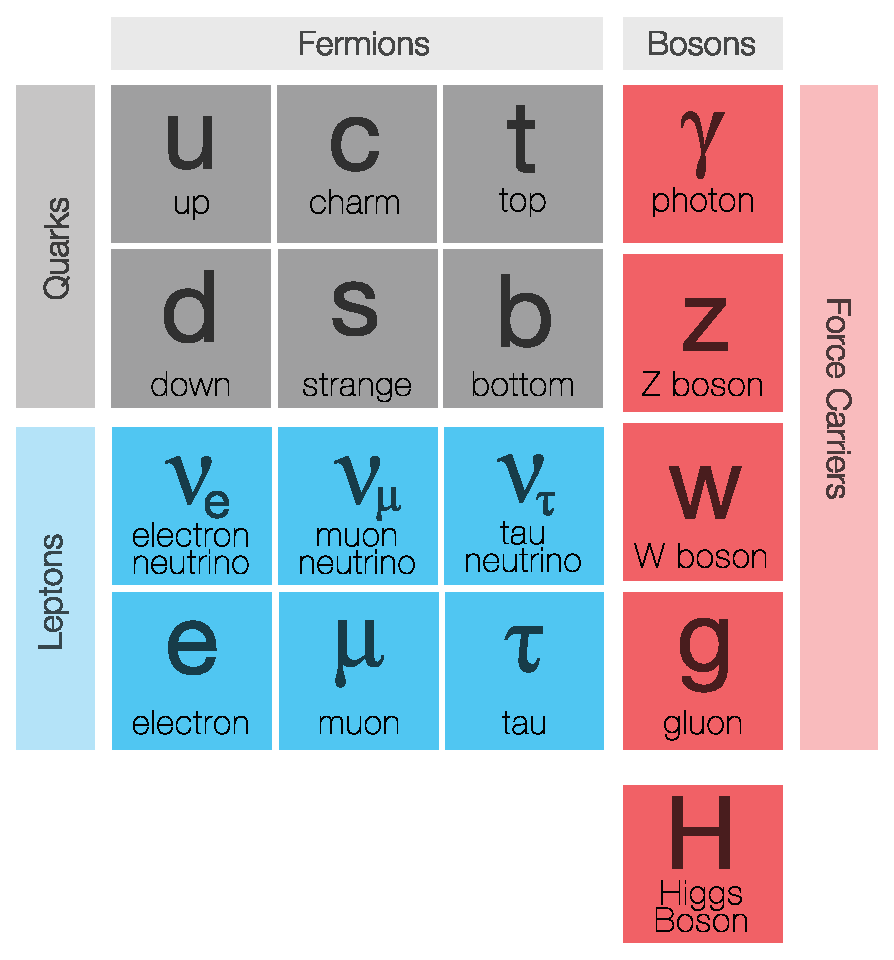
\includegraphics[width=0.28\textwidth]{standard_model}
		\caption{The Standard Model}
		\label{fig:SM}
	\end{wrapfigure}
	\filler
	\newpage

	\begin{table}[H]
		\centering
		\caption[Summary of Particle Discoveries]{A summary of particle discoveries. There are distinct error bars on each of the reported masses that I have not included here, but the values in this table are current as of 2012. Particle masses are taken from the Particle Data Group \cite{PDG}, except for that of the Proton, Antiproton, and Neutron, which come from another source \cite{proton_mass} and are current as of 2010.}
		\label{table:particleList}
			\begin{tabular}{lcccl}
				\toprule
				Particle Name & Symbol & Mass & Year & Credit \\
				\midrule
				Photon 				& \HepParticle{\Pphoton} 		& 0 				& --- 		& --- \\
				Electron 			& \HepParticle{\Pelectron}		& \mMeV{5.486} 		& 1897 		& J.J. Thomson \\
				Proton 				& \HepParticle{\Pproton}		& \mMeV{938.3}		& 1919		& Ernest Rutherford \\
				Neutron 			& \HepParticle{\Pneutron}		& \mMeV{939.6}		& 1932		& James Chadwick \\
				Positron			& \HepParticle{\APelectron}		& \mMeV{5.486}		& 1932		& Carl D. Anderson \\
				Muon				& \HepParticle{\Pmu}			& \mMeV{105.7} 		& 1937 		& Seth Neddermeyer, et al. \\
				Pion 				& \HepParticle{\Ppi}			& \mMeV{135.0}		& 1947		& C. F. Powell, et al. \\
				Kaon 				& \HepParticle{\PK}				& \mMeV{497.6}		& 1947		& George Dixon, et al. Rochester \\
				Lambda Baryon		& $\Lambda^0$					& \mMeV{1116}		& 1950		& V D Hopper, et al. \\
				Antiproton			& \HepParticle{\APproton}		& \mMeV{938.3}		& 1955		& Owen Chamberlain, et al. \\
				Electron Neutrino 	& \HepParticle{\Pnue}			& $<$ \mmeV{2}		& 1956		& Frederick Reines \& Clyde Cowan \\
				Muon Neutrino 		& \HepParticle{\Pnum}			& $<$ \mmeV{190}	& 1962		& Leon Lederman, et al. \\
				Xi Baryon 			& $\Xi^0$						& \mMeV{1315} 		& 1964		& Brookhaven National Laboratory \\
				Up Quark 		 	& u 							& \mMeV{2.3}		& 1969 		& SLAC \\
				Down Quark 		 	& d  							& \mMeV{4.8}		& 1969 		& SLAC \\
				Strange Quark 		& \HepParticle{\Pstrange}		& \mMeV{95}			& 1969 		& SLAC \\
				J$/ \psi$ Meson		& \HepParticle{\PJpsi}			& \mMeV{3097}		& 1974		& Burton Richter, et al. \\
				Charm Quark 		& \HepParticle{\Pcharm} 		& \mGeV{3.45}		& 1974 		& Burton Richter, et al. \\
				Tau 				& \HepParticle{\Ptau}			& \mMeV{1777}		& 1975		& Martin Perl, et al. \\
				Upsilon Meson 		& $\Upsilon$					& \mMeV{9460} 		& 1977		& Fermilab \\
				Bottom Quark 		& \HepParticle{\Pbottom}		& \mGeV{4.18} 		& 1977 		& Fermilab \\
				Gluon				& \HepParticle{\Pgluon}			& 0 				& 1979		& DESY \\
				W Boson 			& W$^{\pm}$ 					& \mGeV{80.39}		& 1983		& Carlo Rubbia, et al. \\
				Z Boson 			& Z$^0$ 						& \mGeV{2.495}		& 1983		& Carlo Rubbia, et al. \\
				Top Quark 			& \HepParticle{\Ptop} 			& \mGeV{173.5}		& 1995		& Fermilab \\
				Tau Neutrino 		& \HepParticle{\Pnut}			& $<$ \mMeV{18.2}	& 2000		& Fermilab \\
				Higgs Boson 		& \HepParticle{\PHiggs} 		& \mGeV{126.0}		& 2012		& CERN (ATLAS) \\				
				\bottomrule
			\end{tabular}
	\end{table}

	\vspace{0.3in}
	\newpage

	\section{The Neutrino and its Properties}

	It was in 1930 that Wolfgang Pauli sought to solve the problem that surrounded $\beta$-decay. The problem was that the process in which a neutron decayed into a proton and an electron seemed to violate the well-established conservation laws of energy, momentum, and spin. Pauli hypothesized the existence of a small neutral particle to reconcile this discrepancy. The idea was a bold one, since the proton and electron were the only two known particles at the time. Neils Bohr opposed Pauli's hypothesis and preferred a statistical explanation that allowed for the violation of conservation laws. Pauli's postulated particle later became known as the neutrino\footnote{More specifically, the electron neutrino. The existence of the other two flavors---the muon neutrino and tau neutrino---were not hypothesized until 1948 and 1974, respectively.}, meaning \emph{little neutral one}.

	Its existence was confirmed in a famous experiment by Fredrick Reines and Clyde Cowan in 1956. They used a mixture of water and cadmium chloride as an interaction medium for electron antineutrinos, which invoke an inverse $\beta$-decay process (\EQ \ref{eq:inv_beta_decay}). 

	\begin{equation}
		\label{eq:inv_beta_decay}
		\HepProcess{\HepParticle{\APnue}{}{} + \HepParticle{\Pproton}{}{} \HepTo \HepParticle{\Pneutron}{}{} + \HepParticle{\Ppositron}{}{}}
	\end{equation}

	The resultant positron quickly annihilates with a nearby electron, producing two $\gamma$ photons. On a larger time scale, the resultant neutron eventually captures on one of the cadmium nuclei, exciting it. When the nucleus de-excites, it emits a photon. Reines and Cowan measured a time delay between detection of the pair-annihilation photons and the neutron capture photon like the theory predicts \cite{first_nu_detection}. \\

	\plan{Discovery of $\mu$ and $\tau$ neutrinos}

		Of all the particles found in nature, neutrinos are perhaps the most ubiquitous. 
		\plan{Mass limits; Neutral charge}

	\subsection{Interactions}

		\begin{wrapfigure}{r}{0.4\textwidth}
			\begin{center}
				\begin{tikzpicture}[
			        thick,
			        % Set the overall layout of the tree
			        level/.style={level distance=1.5cm},
			        level 2/.style={sibling distance=2.6cm},
			        level 3/.style={sibling distance=2cm}
				    ]
				    \coordinate
				        child[grow=left]{
				            child {
				                node {$e^-$}
				                % The 'edge from parent' is actually not needed because it is
				                % implicitly added.
				                edge from parent [fermion-out]
				            }
				            child {
				                node {$\nu_e$}
				                edge from parent [fermion-in]
				            }
				            edge from parent [photon] node [above=3pt] {$W$}
				        }
				        % I have to insert a dummy child to get the tree to grow
				        % correctly to the right.
				        child[grow=right, level distance=0pt] {
				        child  {
				            node {$n$}
				            edge from parent [fermion-in]
				        }
				        child {
				            node {$p$}
				            edge from parent [fermion-out]
				        }
				    };

				\end{tikzpicture}
			\end{center}
			\caption[A Feynman Diagram]{This Feynman diagram is not properly placed yet. Just using this as a test and storage place of the TikZ code to produce diagram.}
			\label{fig:feynman}
		\end{wrapfigure}

		\plan{Neutral current and charged current interactions}

	\subsection{Oscillatory Behavior}

		\plan{Mass and flavor eigenstates; Mixing matrix}

		\plan{Current and past experiments}

		\plan{Vacuum vs matter oscillations}


%-----------------------------------------------------------------------------
%-----------------------------------------------------------------------------